\documentclass[12pt, spanish]{article}
\usepackage[spanish]{babel}
\selectlanguage{spanish}
\usepackage{natbib}
\usepackage{url}
\usepackage[utf8x]{inputenc}
\usepackage{graphicx}
\graphicspath{{images/}}
\usepackage{parskip}
\usepackage{fancyhdr}
\usepackage{vmargin}


\usepackage{tikz}
\usepackage{amsfonts}


\usepackage{hyperref}
\usepackage[
    type={CC},
    modifier={by-nc-sa},
    version={4.0},
]{doclicense}

\hypersetup{
    colorlinks=true,
    linkcolor=blue,
    filecolor=magenta,      
    urlcolor=cyan,
}

\usepackage[default]{sourcesanspro}

\setmarginsrb{2 cm}{1 cm}{2 cm}{2 cm}{1 cm}{1.5 cm}{1 cm}{1.5 cm}

\title{Modelos de Computación:\\
Práctica 4. \hspace{0.05cm} }                           
\author{Antonio David Villegas Yeguas}                             
\date{\today}                                           

\renewcommand*\contentsname{hola}

\makeatletter
\let\thetitle\@title
\let\theauthor\@author
\let\thedate\@date
\makeatother

\pagestyle{fancy}
\fancyhf{}
\rhead{\theauthor}
\lhead{\thetitle}
\cfoot{\thepage}

\begin{document}
%%%%%%%%%%%%%%%%%%%%%%%%%%%%%%%%%%%%%%%%%%%%%%%%%%%%%%%%%%%%%%%%%%%%%%%%%%%%%%%%%%%%%%%%%

\begin{titlepage}
    \centering
    \vspace*{0.5 cm}
    
\includegraphics[scale = 0.50]{ugr.png}\\[1.0 cm]
    %\textsc{\LARGE Universidad de Granada}\\[2.0 cm]   
    \textsc{\large 3ºA - A2}\\[0.5 cm]            
    \textsc{\large Grado en Ingeniería Informática}\\[0.5 cm]              
    \rule{\linewidth}{0.2 mm} \\[0.2 cm]
    { \huge \bfseries \thetitle}\\
    \rule{\linewidth}{0.2 mm} \\[1 cm]
    
    \begin{minipage}{0.4\textwidth}
        \begin{flushleft} \large
            \emph{Autor:}\\
            \theauthor
            \end{flushleft}
            \end{minipage}~
            \begin{minipage}{0.4\textwidth}
            \begin{flushright} \large
            \emph{Asignatura: \\
            Modelos de Computación}                   
        \end{flushright}
    \end{minipage}\\[0.5cm]
  
    {\large \thedate}\\[0.5cm]
    {\url{https://github.com/advy99/MC/}}
    {\doclicenseThis}
 	
    \vfill
    
\end{titlepage}

%%%%%%%%%%%%%%%%%%%%%%%%%%%%%%%%%%%%%%%%%%%%%%%%%%%%%%%%%%%%%%%%%%%%%%%%%%%%%%%%%%%%%%%%%

%\tableofcontents
%\pagebreak

%%%%%%%%%%%%%%%%%%%%%%%%%%%%%%%%%%%%%%%%%%%%%%%%%%%%%%%%%%%%%%%%%%%%%%%%%%%%%%%%%%%%%%%%%

\section{Ejercicio 1:} Obtener un AFD capaz de aceptar las cadenas u ∈ {0,1}* que contengan simultáneamente las subcadenas 000 y 111 haciendo uso del autómata producto.

Primero obtenemos el AFD capaz de aceptar las subcadenas 000.

\begin{center}
	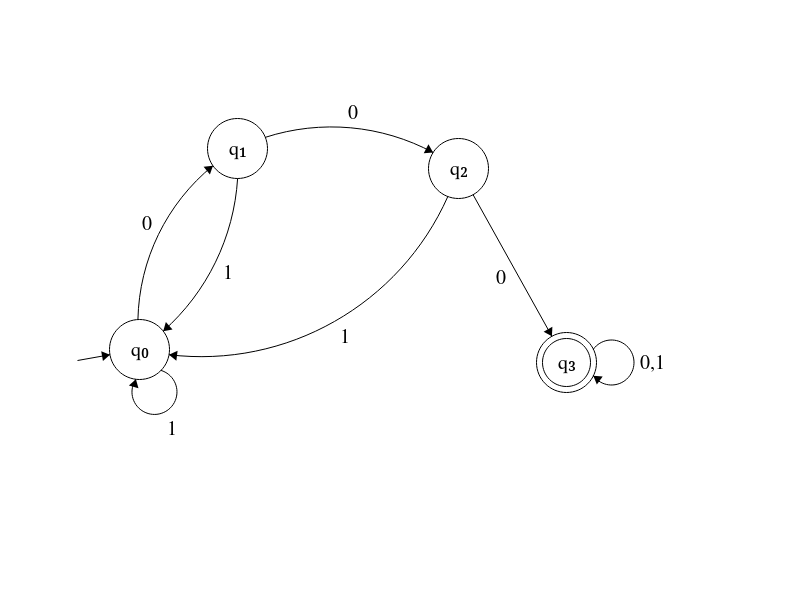
\includegraphics[scale=0.45]{aut1.png}
\end{center}

Ahora obtenemos el AFD capaz de aceptar las subcadenas 111.

\begin{center}
	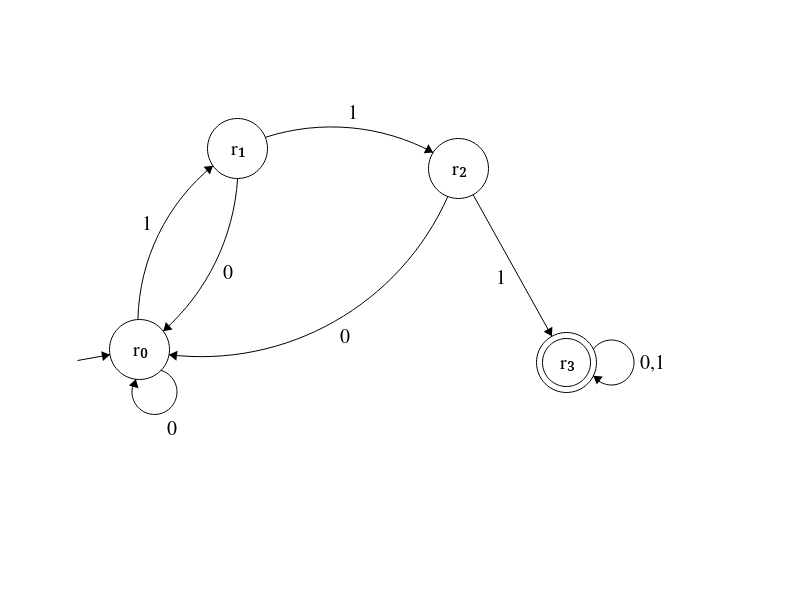
\includegraphics[scale=0.45]{aut2.png}
\end{center}

\newpage

A partir de estos dos AFD calcularemos el autómata producto:


\begin{center}
	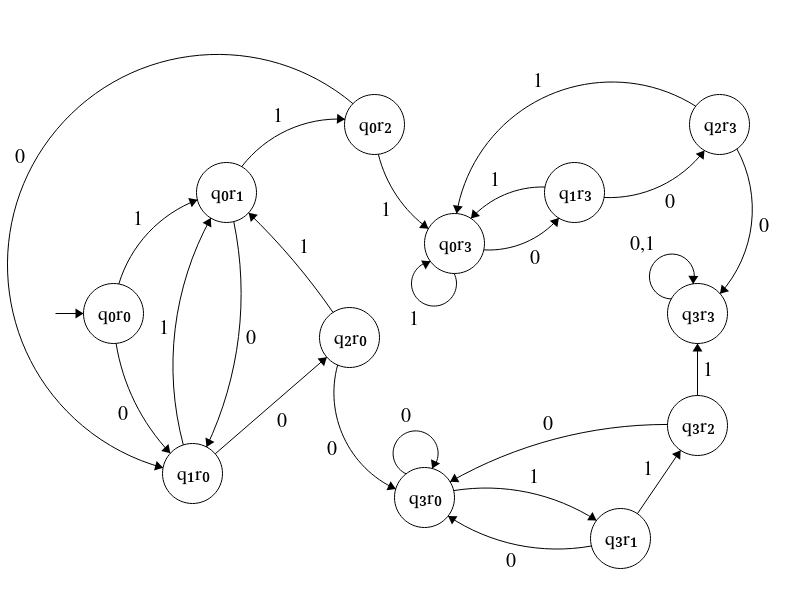
\includegraphics[scale=0.45]{aut_pro.png}
\end{center}

Como nos pide que contenga ambas cadenas, buscamos el autómata intersección, que se consigue haciendo que los estados finales del autómata producto sean los estados en los que solo están los estados finales de los autómatas por separado, es decir, los estados que contenga $q_3$ y $r_3$.

\begin{center}
	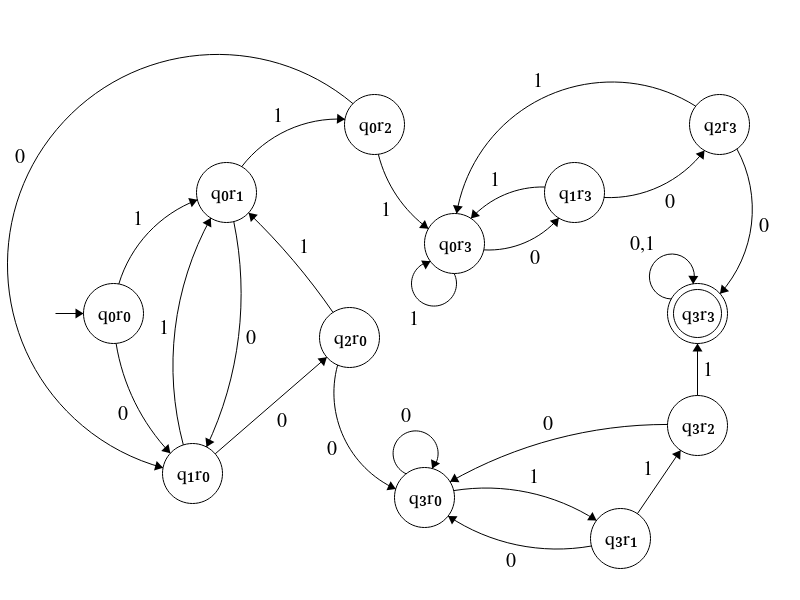
\includegraphics[scale=0.45]{aut_inter.png}
\end{center}


\section{Ejercicio 2:} Calcular el autómata minimal que acepta el mismo lenguaje que el siguiente autómata:

\begin{center}
	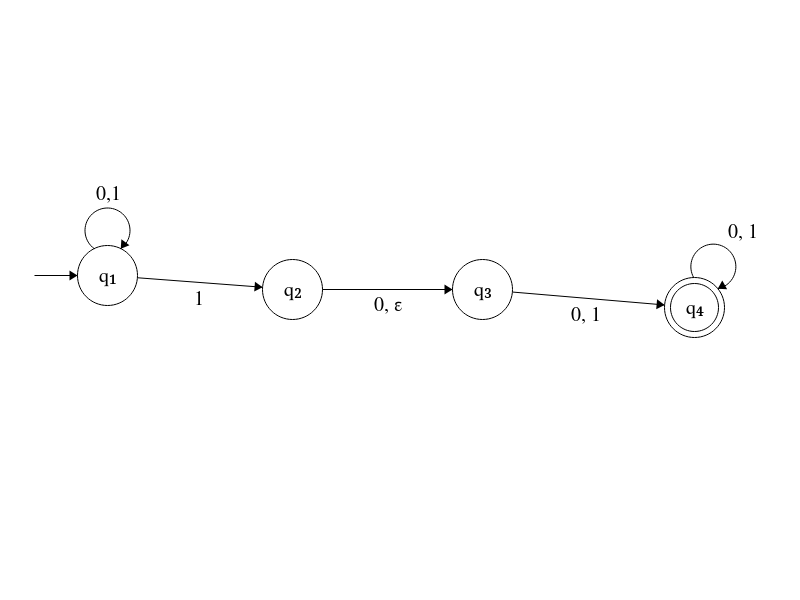
\includegraphics[scale=0.45]{enun2.png}
\end{center}

El primer paso para calcular el autómata minimal será pasar este autómata no determinístico con transiciones nulas a un autómata finito determinístico sin transiciones nulas.

Aplicando el algoritmo visto tanto en teoría como en prácticas, obtenemos el siguiente autómata:


\begin{center}
	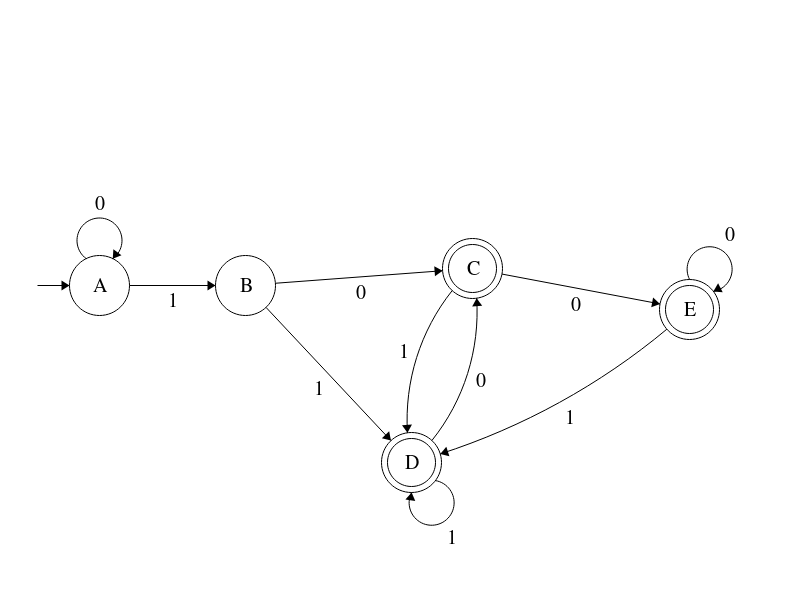
\includegraphics[scale=0.45]{finito2.png}
\end{center}

Siendo:

\begin{enumerate}
	\item A el estado $q_1$.
	\item B el estado $\{q_1, q_2, q_3\}$.
	\item C el estado $\{q_1, q_3, q_4\}$.
	\item D el estado $\{q_1, q_2, q_3, q_4\}$.
	\item E el estado $\{q_1, q_4\}$.
\end{enumerate}

Ahora pasamos a la minimización del autómata finito determinístico.

Separamos los estados en dos conjuntos, finales y no finales, por lo que tendremos la siguiente separación:

\begin{enumerate}
	\item A y B.
	\item C, D y E.

\end{enumerate}


Para empezar, comprobaremos si A y B son equivalentes:

El estado A al leer un 0 pasa al estado A (no cambiamos de conjunto).

El estado A al leer un 1 pasa al estado B (no cambiamos de conjunto).

El estado B al leer un 0 pasa al estado C (cambiamos de conjunto).

El estado B al leer un 1 pasa al estado D (cambiamos de conjunto).

Como vemos, A y B no son equivalentes, ya que en sus transiciones no van al mismo conjunto.

Pasamos a tener los siguientes conjuntos:

\begin{enumerate}
	\item A.
	\item B.
	\item C, D y E.

\end{enumerate}

Pasamos a comprobar si C y D son equivalentes:

El estado C al leer un 0 pasa al estado E (no cambiamos de conjunto).

El estado C al leer un 1 pasa al estado D (no cambiamos de conjunto).

El estado D al leer un 0 pasa al estado C (no cambiamos de conjunto).

El estado D al leer un 1 pasa al estado D (no cambiamos de conjunto).


Como vemos, C y D son equivalentes, ya que en sus transiciones van al mismo conjunto.

Mantenemos los mismos conjuntos.

Pasamos a comprobar si C y E son equivalentes:

El estado C al leer un 0 pasa al estado E (no cambiamos de conjunto).

El estado C al leer un 1 pasa al estado D (no cambiamos de conjunto).

El estado E al leer un 0 pasa al estado E (no cambiamos de conjunto).

El estado E al leer un 1 pasa al estado D (no cambiamos de conjunto).

Como vemos, C y E son equivalentes, ya que en sus transiciones van al mismo conjunto.


Por lo que finalmente tenemos estos conjuntos:


\begin{enumerate}
	\item A.
	\item B.
	\item C, D y E.

\end{enumerate}

Así que podemos decir que C, D y E son el mismo estado, obteniendo el siguiente autómata:

\begin{center}
	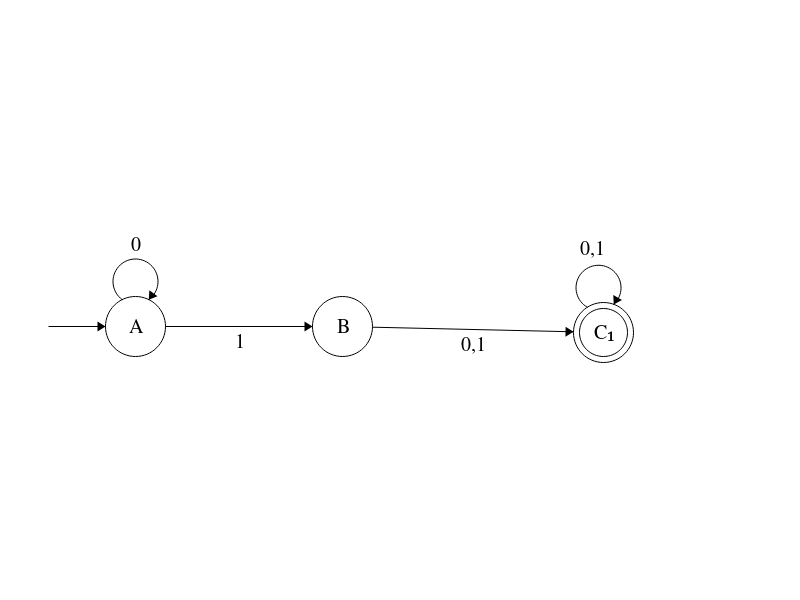
\includegraphics[scale=0.45]{minimizado.png}
\end{center}

\newpage

\section{Ejercicio 3: Indicar si los siguientes lenguajes son o no regulares:}

Para comprobar si los siguientes lenguajes son regulares o no utilizaremos el lema de bombeo. Todo lenguaje regular cumple el lema de bombeo, por lo que si el lenguaje no cumple el lema de bombeo, podemos asegurar que no es regular.

Debemos tener cuidado, porque hay lenguajes no regulares que si cumplen el lema de bombeo, así que si un lenguaje cumple este lema, no podemos asegurar que sea regular.

El lema de bombeo dicta lo siguiente:

Sea L un conjunto regular, entonces $\exists n \in \mathbb{N}$ tal que $\forall z \in $, si $|z| \geq n$, entonces z se puede expresar de la forma z = uvw donde:

\begin{enumerate}
	\item $|uv| \leq n$
	\item $|v| \geq 1$
	\item $(\forall i \geq 0) uv^iw \in L$
\end{enumerate} 


Por lo que para comprobar si un lenguaje no es regular, negaremos el lema de bombeo sobre el lenguaje L:

Sea L un conjunto regular, entonces $\forall n \in \mathbb{N}$ tal que $\exists z \in L$, si $|z| \geq n$, entonces $\forall z = uvw$ donde:


\begin{enumerate}
	\item $|uv| \leq n$
	\item $|v| \geq 1$
	\item $(\exists i \geq 0) uv^iw \not \in L$
\end{enumerate} 


\subsection{}
 $L_1 = \{ (aa)^nb^{m+1} \in \{a,b\}^* $ tal que  $n >= 0, m >= n\}$.


Primero, para cualquier n tenemos que escoger una palabra z que pertenezca al lenguaje. Yo escogeré la siguiente palabra: $z = (aa)^nb^{n+1}$. Como vemos, esta palabra esta dentro del lenguaje, ya que $(aa)$ aparece n veces y $b$ aparece $n+1$ veces.

Por el lema de bombeo, podemos descomponer z en:

\begin{enumerate}
	\item $u = (aa)^k$
	\item $v = (aa)^l$
	\item $w = (aa)^{n - l - k}b^{n+1}$
\end{enumerate}

Por lo tanto, $\exists i$ tal que $uv^iw \not \in L_1$

\newpage

Vemos como:
	$$uv^iw = (aa)^k(aa)^{li}(aa)^{n-l-k}b^{n+1}$$ 
	$$ =  (aa)^{n - l - k + k + li}b^{n+1} $$
	$$ =  (aa)^{n - l  + li}b^{n+1}$$
	$$ =  (aa)^{n + l(i - 1)}b^{n+1}  $$

Por lo que si escogemos $i = 2$, como $|v| \geq 1$ entonces $l \geq 1$, luego $n+l \geq n+1$, por lo que $uv^iw \not \in L_1$

Por lo tanto, podemos asegurar que el lenguaje no es regular ya que no cumple el lema de bombeo.


\subsection{}
 $L_2 = \{ ww $ tal que  $ w \in \{0,1\}^* \}$.
 
Primero, para cualquier n tenemos que escoger una palabra z que pertenezca al lenguaje. Yo escogeré la siguiente palabra: $z = 0^n10^n1$. Como vemos, esta palabra esta dentro del lenguaje, ya que $0^n1$ se repite dos veces.

Por el lema de bombeo, podemos descomponer z en:

\begin{enumerate}
	\item $u = 0^k$
	\item $v = 0^l$
	\item $w =0^{n - l - k}10^n1$
\end{enumerate}

Por lo tanto, $\exists i$ tal que $uv^iw \not \in L_2$

Vemos como:
	$$uv^iw = 0^k0^{li}0^{n-l-k}10^n1$$ 
	$$ =  0^{n - l - k + k + li}10^n1 $$
	$$ =  0^{n - l  + li}10^n1$$
	$$ =  0^{n + l(i - 1)}10^n1  $$

Por lo que si escogemos $i = 2$, como $|v| \geq 1$ entonces $l \geq 1$, luego $n+l \geq n$, por lo que en la primera parte tenemos más ceros que la segunda parte, haciendo que $uv^iw \not \in L_2$.

Por lo tanto, podemos asegurar que el lenguaje no es regular ya que no cumple el lema de bombeo.


 \subsection{}
 $L_3 = \{ a^{2^n} \in \{a\}^{*} $ tal que  $ n >= 0 \}$.

Primero, para cualquier n tenemos que escoger una palabra z que pertenezca al lenguaje. Yo escogeré la siguiente palabra: $z = a^{2^n}$. Como vemos trivialmente, esta palabra esta dentro del lenguaje.

Por el lema de bombeo, podemos descomponer z en:

\begin{enumerate}
	\item $u = a^k$
	\item $v = a^l$
	\item $w =a^{2^n - l - k}$
\end{enumerate}

Por lo tanto, $\exists i$ tal que $uv^iw \not \in L_3$

Vemos como:
	$$uv^iw = a^ka^{li}a^{2^n - l - k}$$ 
	$$ =  a^{2^n - l - k + k + li}$$
	$$ =  a^{2^n - l  + li}$$
	$$ =  a^{2^n + l(i - 1)} $$
	

Por lo que si escogemos $i = 2$, como $|uv| \leq n$ y $|v| \geq 1$ entonces $l \geq 1$, por lo tanto, $2^n < 2^n+l < 2^{n+1}$, como resultado, el número de $a$ no sería un cuadrado de 2, haciendo que $uv^iw \not \in L_2$.

Por lo tanto, podemos asegurar que el lenguaje no es regular ya que no cumple el lema de bombeo.

\end{document}

